\documentclass {article}
\usepackage{graphicx}
\usepackage{amsmath}
\usepackage{amssymb}
\usepackage{xcolor}


\renewcommand\vec{\mathbf}
\let\OldS\nabla
\renewcommand{\nabla}{\boldsymbol{\OldS}}

\let\OldHat\hat
\renewcommand{\hat}[1]{\OldHat{\mathbf{#1}}}

% \newcommand{\comment}[1]{}

\newcommand{\comment}[1]{\textcolor{gray}{\small\textit{Comment: #1}}}


\begin{document}
	\thispagestyle{empty}% empty header/footer

	
\begin{center}\strut
	\bfseries\Huge
	What if  Mass Eats the Vacuum? 

\end{center}

	\comment{Does Mass Eat the Vacuum? (Seems like less words)}

\centerline{David Plotz}


\begin{center}\strut
	\date{\today}
\end{center}
\vfill

	
\newpage
\begin{abstract}
	This paper introduces a classical field theory of gravity built on the Maxwell equations and a central physical hypothesis: that mass absorbs zero-point radiation, inducing a net inward momentum flow. Drawing from stochastic electrodynamics (SED), we assume a Lorentz-invariant radiation field present throughout space and hypothesize that mass acts as a sink for this field.  We construct a consistent model of a massive particle, demonstrate energy and momentum conservation, and show that classical tests of general relativity, inlcuding Mercury's precession, gravitational lensing, and gravitational redshift, are reproduced to leading order. This approach provides a novel, Lorentz-invariant, classical alternative to general relativity, and lays a foundation for further exploration.
\end{abstract}
\newpage

\section{Introduction}

 Modern physics rests on two towering achievements: the Standard Model, underpinned by the Dirac equation, and general relativity, based on Einstein’s field equations. One governs the small, the other the large. Each is remarkably successful in its domain.

But they don’t fit together. When applied simultaneously, the equations break down and yield infinities.  Proposals like string theory offer elegant mathematics but few concrete predictions. Despite nearly a century of effort, no unifying framework has emerged. A fresh approach is warranted.

This paper proposes that fresh approach. Rather than quantizing Einstein’s field equations or geometrizing the Dirac equation, we suggest something simpler and stranger: what if mass eats the vacuum?

More precisely, we hypothesize that mass acts as a \emph{sink} for zero-point radiation, a background field that is assumed to pervade all of space.

\comment{TODO: Add a note here or later that the current model uses a heuristic (a “bug”) to regulate the mass–field interaction.}



\subsection{Roadmap}

This paper is structured to follow the logic of the scientific method: we begin with a hypothesis, outline the physical assumptions that support it, explore its mathematical consequences, compare its predictions to experiment, and finally examine whether it offers a deeper conceptual shift.

In \textbf{Section 2}, we introduce the core hypothesis: that mass acts as a sink for momentum from a pervasive background radiation field. We first present the idea intuitively, anchoring the theory in a physical picture, and then spell it out mathematically.

In \textbf{Sections 3 and 4}, we lay out the two core assumptions underlying the hypothesis. By “assumptions,” we mean elements already present in the scientific literature, perhaps unconventional but not novel to this work.\textbf{Section 3} adopts a Maxwell-style framework for gravity. \textbf{Section 4} introduces the zero-point radiation field as the physical manifestation of the vacuum.

\textbf{Sections 5 and 6} contain the technical core of the paper. We introduce two natural cutoffs, in space and frequency, that regulate the mass–field interaction and ensure physical consistency. 

\textbf{Sections 5 and 6} contain the technical core of the paper. We introduce two natural cutoffs, in space and frequency, to regulate the mass–field interaction and ensure physical consistency. A heuristic inspired by Fourier analysis is used to estimate key observables. We then examine whether the inflow of radiation can stabilize mass against gravitational self-energy, and demonstrate conservation of energy and momentum.

In \textbf{Section 7}, we test the theory against observation. We demonstrate that it reproduces the classical predictions of general relativity to leading order: perihelion precession, gravitational lensing, and redshift.

Finally, in \textbf{Section 8}, we turn to the most surprising result: the field equations, when transformed through a mathematical duality, yield the Dirac equation. A single classical theory thus encompasses gravity, electromagnetism, and quantum behavior, without invoking quantization.

\textbf{Section 9} concludes with a discussion of open questions, potential avenues for further investigation, and the broader implications of the framework proposed here.

\section{The Core Hypothesis}

In this section, we introduce our core hypothesis. We want to take a brief moment here to discuss the difference between what I mean by hypothesis and assumption. 

Assumption = someone else's theory, even if kind of fringe

Hypothesis = my theory

\comment{I don't like the word "core" here ... but not sure what to replace it with}

Every theory begins with a hypothesis. If it yields interesting physics and does not contradict experiment, it deserves to be taken seriously. The history of science is full of ideas that sounded outlandish at first but reshaped our understanding. The burden is not on the hypothesis to sound reasonable; it’s on the results to be meaningful.  Here we first present the hypothesis intuitively, anchoring the theory in a physical picture, and then spell it out mathematically.


\subsection{A Physical Picture: Radiation Sink Intuition }
\label{subsec:intuition}

Before introducing equations, we present a simple physical picture to guide intuition. Consider a neutral, perfectly conducting iron sphere, heated until it glows red. When placed in the vacuum of space, it emits infrared radiation and cools down, eventually approaching absolute zero.

But even at zero Kelvin, space is not truly empty. Both classical and quantum theories suggest the presence of a background electromagnetic field—commonly called the zero-point radiation field. "Zero-point" refers to zero-temperature; "radiation" in this context means light. A fuller treatment of this will be offered in \textbf{Section 4}. For now, it is enough to imagine a low-level radiation noise present even in the coldest vacuum. The mass absorbs radiation from this ambient field.

The hypothesis proposed here is that mass absorbs energy from the zero-point field even at absolute zero. This interaction produces a net inward flow of momentum toward the mass.

The remainder of the paper builds from this intuition and develops the consequences of this idea.

 \comment{From a later section, but perhaps we should add it here: This stands in contrast to general relativity, where mass is treated as a cold object sitting in empty space and curving spacetime around it.}

\comment{Optional note: The assumption that mass sinks radiation is implicit in the Feynman Lectures. ... but we are making it our "core" hypothesis?}

\subsection{Core Hypothesis: The Math}

The image above anchors the theory.

If mass always interacts with the zero-point field, then this interaction must have physical consequences. We propose it manifests as an inward-pointing momentum density:

\begin{equation}
\boxed{\vec{P}(r) = -\hat{r} \frac{G m \hbar}{r^2}}
\label{eq:hypothesis}
\end{equation}


A photon traveling through this field experiences a cumulative momentum shift:

\begin{equation}
\Delta \vec{p} = \int_{\text{path}} \vec{P}(r) \, dl
\label{eq:hypothesis2}
\end{equation}

This is our core hypothesis, and its implications will be tested in \textbf{Section 7}.

This is a proposed hypothesis: mass creates a momentum flux capable of acting on radiation. 

Here, in the current iteration of this paper, we simply state the hypothesis and explore its consequences. In future drafts or subsequent work, we hope to derive this form directly from the two assumptions laid out in the next sections.

A few questions are prompted by this hypothesis: Can such a flow obey conservation of energy and momentum? Can it stabilize mass against collapse? Can it account for known gravitational phenomena?

\section{Maxwell-Like Equations for Gravity}

In this section we introduce the first of our two assumptions. We assume that gravity obeys the same set of  equations as that that governs electromagntism, up to a numeric factor in the coupling constant. While the Maxwell equations were originally written for charge and charge currents, we replace these with mass and  mass currents acting as sources.  In natural units (\( c = 1 \)):

\comment{This was chat's version: Our gravitational field theory begins with a structural analogy: just as electromagnetism is governed by Maxwell's equations, we propose that gravity obeys a similar set of vector field equations.  These equations follow the form of Maxwell's equations in electromagnetism, but with mass and mass current acting as sources rather than charge and electric current.}

\begin{equation}
\begin{aligned}
\nabla \times \vec{B} - \partial_t \vec{E} &= -4 \pi G \vec{J}, \quad 
&\nabla \times \vec{E} + \partial_t \vec{B} &= 0 \\
\nabla \cdot \vec{E} &= -4 \pi G \rho, \quad 
&\nabla \cdot \vec{B} &= 0
\end{aligned}
\end{equation}


These equations describe a vector field sourced by mass density \( \rho \) and mass current \( \vec{J} \), with \( G \) playing the role of the coupling constant. 

Some may be surprised by the presence of \( \vec{B} \), a magnetic-like field. But this emerges naturally: just as a moving charge generates a magnetic field, a moving mass generates a “gravitomagnetic” field. While static masses generate only \( \vec{E}\), moving masses induce \( \vec{B} \); however, the effect is negligible unless the mass is both extremely large and rapidly moving. \textbf{Section 7} discusses a physical manifestation of this effect and explores its potential testability..

\subsection{Irrotational and Solenoidal Decomposition}

Any vector field can be split into irrotational (curl-free) and solenoidal (divergence-free) components:

\begin{equation}
\vec{V} = \vec{V}_I + \vec{V}_S, \quad 
\nabla \cdot \vec{V}_S = 0, \quad 
\nabla \times \vec{V}_I = 0
\end{equation}

Applying this to our gravitational fields yields two decoupled subsystems:

\vspace{0.5em}
\noindent\textbf{Static Fields (Irrotational):}

\begin{equation}
\nabla \cdot \vec{E}_I = -4 \pi G \rho, \quad 
\partial_t \vec{E}_I = 4 \pi G \vec{J}_I, \quad 
\nabla \cdot \vec{J}_I + \partial_t \rho = 0
\end{equation}

\noindent\textbf{Radiation Fields (Solenoidal):}


\begin{equation}
\nabla \times \vec{B}_S - \partial_t \vec{E}_S = 4 \pi G \vec{J}_S, \quad 
\nabla \times \vec{E}_S + \partial_t \vec{B}_S = 0
\end{equation}

This decomposition reflects a meaningful physical distinction between the \textbf{static gravitational attraction} and the \textbf{propagating radiation} field.

In the rest frame of the mass, these sectors decouple. One set of equations governs the gravitational field sourced by the mass, while another describes the radiation field. This separation enables a detailed analysis of radiation without affecting the static component.

We can make this explicit by defining a new current:


\begin{equation}
\vec {J_S'} = - G \vec {J_S}
\end{equation}

This transforms the inhomogeneous solenoidal equation into:

\begin{equation}
\nabla \times \vec B_S - \partial_t \vec E_S =  4 \pi \vec {J_S'}
\end{equation}

while leaving all other equations unchanged.

Since this form matches the standard presentation in textbooks on electromagnetic radiation, we will drop the prime and adopt the following as the solenoidal (radiation) Maxwell equations:

\begin{equation}
\begin{aligned}
\nabla \times \vec B_S - \partial_t \vec E_S =  4 \pi \vec J_S \\
\nabla \times \vec E_S + \partial_t \vec B_S = 0 
\end{aligned}
\end{equation}

\subsection{Spherical Vector Harmonics}

The following sections derive the explicit solutions to the Maxwell equations used in this theory.

Due to the symmetric radial symmetry of the problem, we will benefit from using Vector Spherical Harmonics. 

Following Berrara (http://iopscience.iop.org/article/10.1088/0143-0807/6/4/014/meta) we assume that any vector field, $\vec V$, and any scalar, $g$, can be expanded as follows:



\begin{align}
\vec{V}(\vec{x}) = \sum_{l=0}^{\infty} \sum_{m=-l}^{l} \big[ 
& a_{lm}(r)\, \vec{Y}_{lm}(\theta, \phi) 
+ b_{lm}(r)\, \hat{r} \times \vec{X}_{lm}(\theta, \phi) \notag \\
& + c_{lm}(r)\, \vec{X}_{lm}(\theta, \phi) 
\big]
\end{align}

\begin{equation}
g(\vec x) = \sum_{l=0}^{\infty} \sum_{m=-l}^{l} g_{lm}(r) Y_{lm}(\theta, \phi)
\end{equation}


where $Y_{lm}$ are the usual spherical harmonics (see Jackson 3.53), $\vec Y_{lm}$ is simply $\hat r Y_{lm}$  and $\vec X_{lm}$ is defined as,


\begin{equation}
\vec X_{lm}(\theta, \phi) = \frac {-i}{\sqrt{l(l+1)}} \vec r \times \left( \nabla Y_{lm}(\theta, \phi) \right) 
\label{eq:xlm}
\end{equation}

\subsection{Recovery of Newtonian Gravity (Irrotational Solutions)}

We now calculate Newtonian gravity as a solution to the Irrotational parts of the Maxwell equations.

In the case of a static point mass \( m \) located at the origin, we set:

\begin{equation}
\rho(\vec{x}) = m \delta^3(\vec{x}), \quad \vec{J} = 0
\end{equation}


Using the irrotational part of the Maxwell equations:


\begin{equation}
\nabla \cdot \vec{E}_I = -4 \pi G \rho ~~~~~~~~~~ \nabla \times \vec{E}_I = 0
\end{equation}

and using the spherical vector harmonics we developed earlier,  we find:


\begin{equation}
\vec E_I(\vec x) = \sum_{l,m} \left[ -\frac {4\pi i G }{2l+1} \frac {q_{lm}}{r^{l+2}} \sqrt {l(l+1)} \left(\hat r \times \vec X_{lm} \right)  - \frac {4 \pi G (l+1)}{2l+1} \frac {q_{lm}}{r^{l+2}} \vec Y_{lm} \right] 
\end{equation}

Where,

\begin{equation}
q_{lm} \equiv \int Y_{lm}^* (\theta, \phi) r^l  \rho (\vec x) ~ d^3x = \int \rho_{lm} (r) r^{l+2} ~ dr 
\end{equation}

Clearly then, if

\begin{equation}
\rho(\vec{x}) = m \delta^3(\vec{x})
\end{equation}


We get

\begin{equation}
\vec E_I(\vec x) = - \hat{r}\frac {mG} {r^2}
\end{equation}

as expected.



\subsection{Radiation from the Solenoidal Field (Solenoidal Solutions)}

Several results from the solutions of the solenoidal Maxwell equations will be needed later; we now solve the corresponding equations.

Outside the mass, the solenoidal field equations in vacuum are:

\begin{equation}
\nabla \times \vec{E}_S + \partial_t \vec{B}_S = 0, \quad 
\nabla \times \vec{B}_S - \partial_t \vec{E}_S = 0
\end{equation}

Assuming time dependence \( e^{-i \omega t} \), the general solution is expanded in vector spherical harmonics:

\begin{equation}
\begin{aligned}
\vec{B}_S &= \sum_{l,m} \left[
a_E(l,m) f_l(kr) \vec{X}_{lm}
- \frac{i}{k} a_M(l,m) \nabla \times \left( g_l(kr) \vec{X}_{lm} \right)
\right] \\
\vec{E}_S &= \sum_{l,m} \left[
\frac{i}{k} a_E(l,m) \nabla \times \left( f_l(kr) \vec{X}_{lm} \right)
+ a_M(l,m) g_l(kr) \vec{X}_{lm}
\right]
\end{aligned}
\end{equation}

where \(\vec{X}_{lm}\) was defined in~\eqref{eq:xlm}.



The functions $f_l$ and $g_l$ are linear superpositions of the radial Hankel functions,

\begin{equation}
h_l^{(1)}(x) = -i (-x)^l \left(\frac 1 x \frac d {dx} \right)^l \left(\frac {e^{ix}} x \right)
\end{equation}

\begin{equation}
h_l^{(2)}(x) = \left( h_l^{(1)}(x) \right)^*
\end{equation}

\noindent $a_E$ and $a_M$ as well as the particular dependence of $f_l$ and $g_l$ on $h_l^{(1)}(x) $ and $h_l^{(2)}(x) $ depend on the boundary conditions.

In our case, we are looking at a massive particle that sinks radiation, we therefore need to only include incoming waves.

The total instantaneous power absorbed is defined as.

\begin{equation}
P \equiv \int_V d^3x ~ \nabla \cdot \left( \frac 1 {8 \pi} \vec E \times \vec B^*\right) = \oint_{\partial V} \hat r \cdot \vec S ~ da = R^2 \int d\Omega ~ \hat r \cdot \vec S \bigg|_{r = R}
\end{equation}

Using the relationships in the introduction on Vector Spherical harmonics, we find that we are left with only two non-vanishing terms,

\begin{equation}
P = \frac {R^2}{8 \pi} \sum_{l, m} \left[  \frac {-i} k |a_E|^2 h_l^{(2)} \frac 1 r \frac d {dr} \left( rh_l^{(1)} \right) + \frac i k |a_M|^2 h_l^{(1)} \frac 1 r \frac d {dr} \left( rh_l^{(2)}\right) \right]_{r=R}
\end{equation}

Since, by assumption (See Section~\ref{subsec:intuition}) the massive particle is electromagnetically neutral on average, we need neither the Transverse Magnetic nor the Transverse Electric modes to dominate. Thus, the two proportionality terms must obey $|a_E|^2 = |a_M|^2$. Use of the Wronskian leaves a particularly simple form for the power radiated,


\begin{equation}
P = \sum_{l,m} \frac {|a_E|^2} { 4 \pi k^2}
\end{equation}

The associated momentum density also follow cleanly. The total field momentum is directed radially inward:

\begin{equation}
\vec{P}_{\text{field}} = \frac{1}{8\pi} \int_V \vec{E} \times \vec{B}^* \, d^3x
= -\hat{r} \sum_{l,m} \int_V \frac{|a_E|^2 |\vec{X}_{lm}|^2}{4\pi k^2 r^2} \, d^3x
\label{eq:mom}
\end{equation}


The above was calculated exactly. However, the total field energy is more difficult to calculate. In the present work we only calculte the energy in the radiation zone: $k^2 r^2  >> 1$. We discuss aspects of this further in ~\ref{subsec:heuristic}. In the radiation zone, we can use the approximation:


\begin{equation}
\begin{aligned}
\vec{B}_S &= \frac {e^{-ikr}} {kr}  \sum_{l,m}  (-i)^{l+1}    \left[
a_E(l,m) \vec{X}_{lm}
+ a_M(l,m) \hat{r} \times  \vec{X}_{lm} 
\right] \\
\vec{E}_S &= \frac {e^{-ikr}} {kr} \sum_{l,m}  (-i)^{l+1}   \left[
a_M(l,m) \vec{X}_{lm}
- a_E(l,m) \hat{r} \times  \vec{X}_{lm} 
\right] 
\end{aligned}
\end{equation}

From this it follows straightforwardly that 


\begin{equation}
U  =\sum_{l, m}   \int_V \frac 1 {4 \pi}  \frac {|a_E|^2 |\vec X_{lm} |^2}{k^2 r^2} ~ d^3x 
\label{eq:energy}
\end{equation}

The expansion of this outside of the radiation zone leads to intriguing math but we must save it for future research .

The specific coefficients \( |a_E|^2 \) will be fixed by boundary conditions in the section ~\ref{sec:stability} on collapse and stability. But, since we've already spelled out the hypothesis several times now, then we know that we will eventually land on
:

\begin{equation}
\boxed{
	\vec{p}(r) = -\hat{r} \frac{G m \hbar}{r^2}
}
\tag{\ref{eq:hypothesis}}
\end{equation}

This result follows from boundary conditions at the mass’s surface.

\comment{We probably need better writing here ... maybe say something about a heuristic ... or something}

\section{Stochastic Electrodynamics (SED)}

To complete our framework, we now introduce our second assumption:  the textbf{zero-point radiation field}. Following the ideas of stochastic electrodynamics (SED), we assume that the vacuum is filled with a classical, Lorentz-invariant electromagnetic radiation field even at absolute zero. 

Historically, the Michelson–Morley experiment aimed to detect the luminiferous aether, the medium through which light was thought to propagate. The null result helped solidify the notion of a truly empty vacuum. In contrast, SED treats the vacuum as filled with fluctuating electromagnetic fields, even at absolute zero.

In SED, zero-point radiation explains how classical systems can remain stable even while radiating energy. It has been shown to reproduce:
\begin{itemize}
	\item The Planck blackbody spectrum (Boyer, 1969) \cite{boyer1969}
	\item Harmonic oscillator ground-state energy \( \tfrac{1}{2} \hbar \omega \) \cite{cole2003}
	\item Casimir and van der Waals forces \cite{boyer1975}
	\item Certain features of the hydrogen atom’s ground state \cite{puthoff1987}
	\item The Unruh effect \cite{boyer1980}
\end{itemize}

Taken together, these results support the view, held by Boyer and others, that the vacuum is in fact an active medium, filled with fluctuating modes that persist even at \( T = 0 \).

Importantly, SED achieves the above results  \emph{without quantization}. All results are derived using classical analysis.


\subsection{The Zero-Point Radiation Field}

In SED, the vacuum is not silent. It carries a random, omnipresent electromagnetic field with spectral energy density:

\begin{equation}
\rho(\omega) = \frac{1}{2} \hbar \omega
\end{equation}

This spectrum is Lorentz-invariant and corresponds to the ground state energy per mode, in analogy to the quantum harmonic oscillator. But unlike quantum theory, which treats this as an abstract baseline, that is generally thrown away or at least ignored, SED models it as a real classical field.

The field is stochastic and Gaussian, defined by:

\begin{equation}
\langle W \rangle = 0, \qquad 
\langle W_i(\vec{k}) W_j^*(\vec{k}') \rangle = \delta_{ij} \delta^3(\vec{k} - \vec{k}')
\end{equation}

The electric and magnetic fields are then:

\begin{equation}
\begin{aligned}
\vec{E}(\vec{x}, t) &= \text{Re} \sum_{\lambda=1}^2 \int d^3k \, 
\hat{\epsilon}(\vec{k}, \lambda) 
\sqrt{\frac{\hbar \omega}{2\pi^2}} 
W_\lambda(\vec{k}) e^{i(\omega t - \vec{k} \cdot \vec{x})} \\
\vec{B}(\vec{x}, t) &= \text{Re} \sum_{\lambda=1}^2 \int d^3k \, 
\frac{\vec{k} \times \hat{\epsilon}(\vec{k}, \lambda)}{k}
\sqrt{\frac{\hbar \omega}{2\pi^2}} 
W_\lambda(\vec{k}) e^{i(\omega t - \vec{k} \cdot \vec{x})}
\end{aligned}
\end{equation}

This background field is homogeneous and isotropic. Each mode contributes an energy \( \tfrac{1}{2} \hbar \omega \), and the full ensemble of modes is statistically stationary and invariant under Lorentz transformations.


The zero-point radiation field plays a central role in the framework. Mass interacts with this field by absorbing momentum from it. This stands in contrast to general relativity, where mass is treated as a cold object sitting in empty space and curving spacetime around it.

\comment{Perhaps we should also state "This stands in contrast to general relativity, where mass is treated as a cold object sitting in empty space and curving spacetime around it" earlier as well ... because it will help with the visualization?  ... I'm putting it into a comment now}




\section{Natural Limits of Mass–Field Interaction}

A central feature of this theory is that mass interacts with the zero-point radiation field only over a constrained domain, bounded by two physically motivated limits: one in space, and one in frequency. These limits are not introduced arbitrarily or for convenience. Rather, they emerge from consistency conditions: the spatial limit prevents runaway collapse, while the frequency limit ensures finite absorption from the radiation field.

Together, they define the natural resolution scale of gravitational interaction. In this section, we outline the arguments for each limit and explore how they might be connected.


\subsection{Lower Bound: Minimum Radius via Gravitational Self-Energy}

From classical considerations, any spherically symmetric mass distribution has a gravitational self-energy:


\begin{equation}
U = -\frac{1}{2} \int \frac{G m \rho(\vec{x})}{r} \, d^3x = E_{\text{nergy}} = m
\end{equation}

For a spherical shell of radius \( R \), this yields:


\begin{equation}
R = \frac{G m}{2}
\end{equation}

Other geometries differ only by numerical prefactors. 

\comment{This is slightly important, because we will be coming back to this in later sections (I will refer to the following equation). The reason it's important is because we are making a model, and the model itself is kind of  ill-definied and fuzzy ... i.e., slightly  different models have different numerical pre-factors ... and the best we can do in tis paper is work with the general magnitude.}

In general, we require:

\begin{equation}
R \gtrsim G m
\end{equation}
\label{radius}

We interpret this as a \textbf{minimum radius} for a stable mass. 

\subsection{Upper Bound: Cutoff Frequency via Energy Matching}

Conversely, we find that we must also impose an upper bound on the frequency components.  A natural upper limit arises from energy conservation:


\begin{equation}
U = m = \hbar \omega_{\text{max}} \quad \Rightarrow \quad \omega \lesssim \frac{m}{\hbar}
\end{equation}


While this frequency is extraordinarily high for macroscopic objects, it plays a crucial theoretical role in regularizing energy and momentum integrals. 

\vspace{0.5em}
Taken together, the cutoffs in radius and frequency define a characteristic resolution scale for gravity. They constrain how mass interacts with the field and suggest a breakdown of classical behavior beyond these limits, potentially pointing toward extensions of the theory. This is also possibly a testable prediction.

\subsection{A Recurring Structure: Observables as Double Integrals}
\label{subsec:heuristic}

Throughout this work, a recurring mathematical structure appears in expressions for physical quantities. These quantities often resist closed-form evaluation, yet they share a distinctive form.

For example, energy and momentum commonly appear as:

\begin{equation}
U = \frac{1}{8\pi^3} \int \int \frac{Gm\hbar}{r^2} \, d^3x \, d^3k
\end{equation}

\begin{equation}
\vec{P}  = - \frac{\hat{r}}{8\pi^3} \int \int \frac{Gm\hbar}{r^2} \, d^3x \, d^3k
\end{equation}

These integrals are rarely evaluated directly. Instead, their structure invites a heuristic move, one that echoes a familiar identity from Fourier analysis:

\begin{equation}
\psi(x) = \int \psi(k) e^{-ikx} \, dk, \quad
\psi(k) = \frac{1}{2\pi} \int \psi(x') e^{ikx'} \, dx'
\end{equation}

Combining these yields:

\begin{equation}
\psi(x) = \frac{1}{2\pi} \int \int \psi(x') e^{ik(x' - x)} \, dk \, dx'
\end{equation}

In such cases, the oscillatory kernel often collapses the integral via delta-function behavior or dominant phase cancellation, without requiring explicit evaluation. The structure itself simplifies the expression.


Similarly, in our case, integrals like those for \(U\) and \(\vec{P}\) often take forms that suggest dominance by a characteristic mode. This leads us to write, heuristically:


\begin{equation}
U \sim \frac{Gm\hbar}{r^2}, \quad
\vec{P}  \sim -\hat{r} \frac{Gm\hbar}{r^2}
\end{equation}

This step is admittedly heuristic, reflecting a structural analogy inspired by Fourier reasoning. While the math is loose, I believe this single approximation shouldn’t discredit the broader theory. In effect, we treat the observable as if it is shaped by the dominant contribution from modes satisfying \(k^2 r^2 \sim 1\), even when we cannot explicitly resolve the integrals.

\comment{Please see the approximation around Jackson (9.128) and later, I refer back to this in an equation as well ... So while this is a ... well this math is super fishy, it is my belief that just this one piece of fishy math shouldn't kill the entire theory}

Whether this reflects true resonance, dimensional filtering, or something deeper remains open.  For now, we emphasize the recurring form and the intuition it offers.





\section{Field Energy and Momentum Balance: A Mechanism for Stability}
\label{sec:stability}



In this section, we examine whether the proposed inflow of zero-point radiation can stabilize a massive particle against gravitational collapse. If the energy absorbed from the vacuum field offsets the divergent self-energy of the particle’s own field, a natural mechanism for stability emerges. We first analyze the energy density and total energy of the system, incorporating a high-frequency cutoff introduced earlier. We then explore whether this energy balance leads to a self-consistent equilibrium. Finally, we turn to momentum conservation, where we derive an effective “Ohm’s law” relating solenoidal fields and currents. Together, these results show that the hypothesized momentum inflow can provide a classical mechanism of stability rooted in the structure of the zero-point field itself.

\subsection{Stability from Field Energy}

We now evaluate whether the inward radiation flow proposed in \textbf{Section 2} can provide a stabilizing mechanism for a massive particle. Specifically, we ask: can the absorbed energy from the zero-point field counterbalance the gravitational self-energy that would otherwise cause collapse?

The total field energy is given by:
\begin{equation}
U = \frac{1}{16\pi} \int \left( |\vec{E}|^2 + |\vec{B}|^2 \right) \, d^3x
\end{equation}

If we pause and look at just the irrotational part of hese equations. we have

\begin{equation}
U_I = \frac{1}{16\pi} \int \left( |\vec{E_I}|^2  \right) \, d^3x
\end{equation}

This leads to 

\begin{equation}
U_I\sim \int \left(\frac { Gm^2} {r^4} \right) \, d^3x
\end{equation}

Which is clearly divergent and therefore a mass would collapse under its own weight without some kind of counter balance force thing.

\comment{Yeah ... I totally used my memory for the above equation, so we should double check it in the next pass}

Unsurprisingly, the hypothesis of this paper is that we should include the radiation contribution, and thus we have:

The total energy, combining both irrotational and solenoidal contributions, is:
\begin{equation}
U_{\text{tot}} = \int_V u \, d^3x = \int_V \left( -\frac{1}{4\pi G} |\vec{E}_I|^2 + |\vec{E}_S|^2 + |\vec{B}_S|^2 \right) \, d^3x
\end{equation}



From equation~\eqref{eq:energy}, we have:
\begin{equation}
U_{\text{rad}} = \sum_{l, m} \int_V \frac{1}{4\pi} \frac{|a_E|^2 |\vec{X}_{lm}|^2}{k^2 r^2} \, d^3x
\end{equation}

And naturally using our hypothesis and the arguments in section  ~\ref{subsec:heuristic} (above about ... getting tired) we then have

\begin{equation}
U_{\text{rad}} =  \frac{1}{8\pi^3} \int \int \frac{Gm \hbar}{r^2} \, d^3x \, d^3k
\end{equation}

Integrating over \(k\) and combining, gives the following total energy:

\begin{equation}
U_{\text{tot}} = \int \left[ \frac{Gm \hbar}{r^2}k^3  - \frac {Gm^2} {r^4}\right] \, d^3x 
\end{equation}


Using the heuristics we developed in subsection ~\ref{subsec:heuristic}, that were admittedly slightly fishy but we had decided were not fatal to the theory, namely that

\begin{equation}
k_{\text{max} }= \frac m {\hbar} ~~~~~~~ and ~~~~ r^2k^2 = 1 
\end{equation}


 we then see that the energy is at most a constant and therefor is conseved 


\subsection{Momentum Conservation and “Ohm’s Law”}

We now turn to momentum conservation. The total momentum exchange in the system should obey:

\begin{equation}
\int_V \left( \rho \vec{E}_I + \vec{J}_S \times \vec{B}_S \right) \, d^3x = 0
\end{equation}


Assuming the solenoidal current obeys a linear response:

\begin{equation}
\vec{J}_S = \sigma \vec{E}_S
\end{equation}

and harmonic time dependence \(e^{-i \omega t}\), the field momentum becomes:

\begin{equation}
-\hat{r} \int \left( m \delta(\vec{x}) \cdot \frac{G m}{r^2} - \sigma \cdot \frac{G m \hbar}{r^2} \right) \, d^3x = 0
\end{equation}

Solving gives:

\begin{equation}
\sigma = \frac{m}{\hbar} \delta(\vec{x})
\end{equation}

This expression defines a delta-function conductivity concentrated at the origin — an effective Ohm's law in which the mass acts as a point-like, perfect absorber for incoming radiation.  We can re-write the relevant Maxwell equation in light of this:

\begin{equation}
\nabla \times \vec{B}_S - \partial_t \vec{E}_S = -\frac{m}{\hbar} \vec{E}_S \delta^3(\vec{x})
\label{eq:ohm}
\end{equation}



Together, the field energy and momentum conservation arguments demonstrate that the hypothesized momentum inflow can act as a self-consistent stabilizing structure. A massive particle that sinks zero-point radiation does not collapse because of the interaction with the vacuum field itself.

	
\section{Classical Tests of Gravity}

This section demonstrates that the present theory reproduces three key experimental predictions of general relativity: the precession of Mercury's perihelion, the deflection of light near a massive object, and gravitational redshift. 

\comment{These are the three classic tests of general relativity ... like pretty sure that Einstein himself propsed these ... or at minimum ... like they're really famous ... we should double check this, and then also mention this up above in the intro and the conclusion} 

\subsection{Precession of the Perihelion of Mercury}

In electrodynamics, a static Coulomb field transforms under Lorentz boosts into a configuration with both electric and magnetic components. Specifically, the fields of a charge moving at velocity \( \vec{v} \) are:

\begin{equation}
\vec{E}' = \gamma \vec{E} - \frac{\gamma^2}{\gamma + 1} \vec{v} (\vec{v} \cdot \vec{E}), \quad
\vec{B}' = - \gamma \vec{v} \times \vec{E}
\end{equation}

where \( \gamma = 1 / \sqrt{1 - v^2} \).

By analogy, we assume the same Lorentz transformation laws apply to gravity. We define the gravitational field:

\begin{equation}
\vec{E}_g = \vec{F} / m = - \frac{G M}{r^3} \vec{r}
\end{equation}

Then, under a Lorentz boost:

\begin{equation}
\vec{E}_g' = \gamma \vec{E}_g - \frac{\gamma^2}{\gamma + 1} \vec{v} (\vec{v} \cdot \vec{E}_g), \quad
\vec{B}_g' = -\gamma \vec{v} \times \vec{E}_g
\end{equation}

In the low-velocity limit \( v \ll 1 \), we find:

\begin{equation}
\vec{B}_g = - \vec{v} \times \vec{r} \cdot \frac{GM}{r^3}
\end{equation}

This introduces a "gravitomagnetic" interaction analogous to magnetism in electrodynamics.

\begin{figure}[t]
	\centering
	\fbox{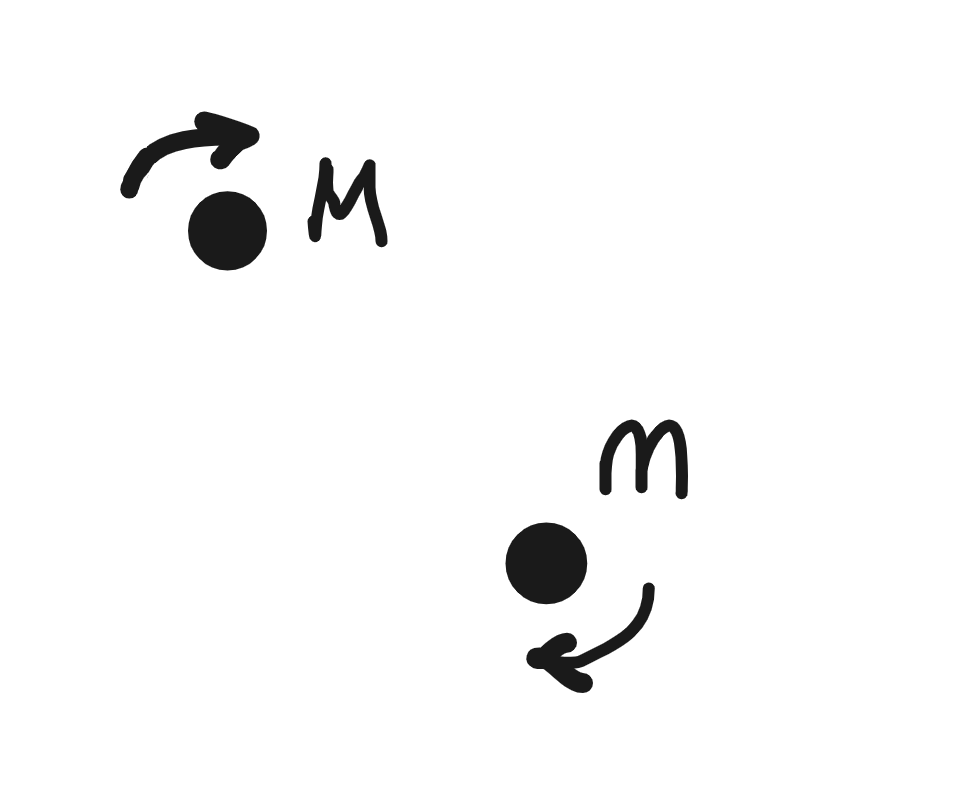
\includegraphics[width=0.6\textwidth]{autodraw.png}}
	\caption{Two masses in mutual orbit}
	\label{fig:two-masses}
\end{figure}

We now consider Kepler’s problem. The Newtonian effective potential is:




\begin{equation}
U_{\text{Newt}} = \frac{1}{2} m \left( \frac{dr}{dt} \right)^2 - \frac{GMm}{r} + \frac{l^2}{2 m r^2}
\end{equation}

where \( l = m |\vec{r} \times \vec{v}| \) is the orbital angular momentum (see Figure \ref{fig:two-masses}).


A moving charge induces a magnetic moment \( \vec{m} = \frac{1}{2} e (\vec{r} \times \vec{v}) \). Replacing \( e \rightarrow m \), we define a gravitational magnetic moment:

\begin{equation}
\vec{m}_g = \frac{1}{2} m (\vec{r} \times \vec{v})
\end{equation}

The potential energy of this moment in a magnetic field is:

\begin{equation}
U = -\vec{m}_g \cdot \vec{B}_g = -\frac{GM m}{2} |\vec{r} \times \vec{v}|^2 / r^3
\end{equation}

This adds a correction to the potential energy. Including the reciprocal effect (from the motion of the central mass), we double this term and find the corrected potential:

\begin{equation}
U_{\text{Einstein}} = \frac{1}{2} m \left( \frac{dr}{dt} \right)^2 - \frac{GMm}{r}
+ \frac{l^2}{2 m r^2} - \frac{GM l^2}{m r^3}
\end{equation}

This is the same correction obtained in general relativity to first order. As Carroll notes, general relativity produces this result exactly; in our theory, it emerges as a first-order approximation. Higher-order terms may offer a route to testing deviations.

\subsection{Deflection of Light}



We now consider the deflection of light near a massive object. Our central hypothesis is that mass creates a momentum-transfer field:

\begin{equation}
\vec{P}(r) = - \hat{r} \frac{G m \hbar}{r^2}
\tag{\ref{eq:hypothesis}}
\end{equation}


\begin{figure}[h]
	\centering
	\fbox{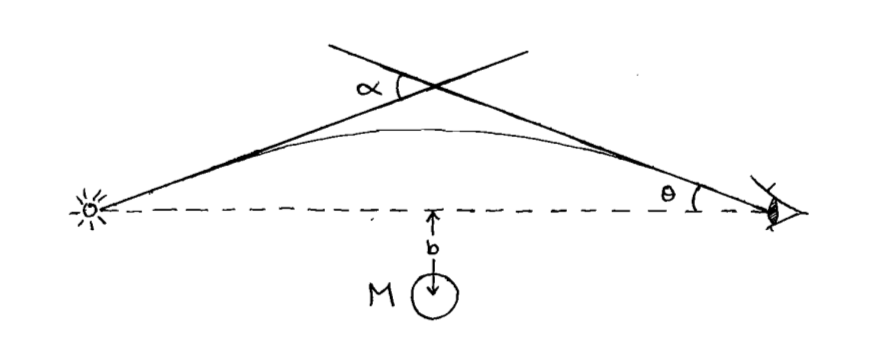
\includegraphics[width=0.6\textwidth]{light-bending.png}}
	\caption{Deflection of light}
	\label{fig:deflection}
\end{figure}

A photon traveling through this field receives a cumulative momentum shift:

\begin{equation}
\Delta \vec{p} = \int_{\text{path}} \vec{P}(r) \, dl
\tag{\ref{eq:hypothesis2}}
\end{equation}

Assuming a straight-line path passing at minimum distance \( b \) (see figure \(\ref{fig:deflection}\)), we integrate:

\begin{equation}
\Delta \vec{p} = \int_{-\infty}^{\infty} - \frac{G m \hbar}{r^3} \vec{r} \, w \, dz
\end{equation}

The parallel momentum shifts cancel symmetrically. The transverse component yields:

\begin{equation}
\Delta p_y = \hbar w \cdot \frac{2 G m}{b}
\end{equation}

The angle of deflection is then:

\begin{equation}
\theta \approx \frac{\Delta p_y}{p_z} = \frac{2 G m}{b} \quad \Rightarrow \quad \alpha = \frac{4 G m}{b}
\end{equation}

This matches, to first-order, the deflection angle predicted by general relativity.

\subsection{Gravitational Redshift}

Finally, we consider the redshift of light climbing out of a gravitational well. As before, a photon gains or loses momentum depending on its path through the momentum field.

Using:

\begin{equation}
\Delta p = \int_{\infty}^{R} \vec{P} \cdot \hat{r} \cdot w \, dr = \int_{\infty}^{R} - \frac{G m \hbar}{r^2} w \, dr = \hbar w \cdot \frac{G m}{R}
\end{equation}

The resulting frequency shift is:

\begin{equation}
\hbar w' = \hbar w + \Delta p = \hbar w \left( 1 + \frac{G m}{R} \right)
\end{equation}

which, to first order, matches the prediction of general relativity for gravitational redshift.

		
\section{Duality and the Dirac Equation}

Throughout this paper, we’ve stayed grounded in classical physics. We built a theory of gravity using field equations, conservation laws, and an underlying sea of vacuum radiation: no quantum assumptions, no curved spacetime. In this section, something surprising appears. When the field equations are rewritten in a new form, a familiar structure emerges: the Dirac equation, the cornerstone of quantum mechanics.

\subsection{Duality Transformations}

As discussed in Jackson (Section 6.11), the Maxwell equations can be extended to include both electric and magnetic charges:

\begin{equation}
\begin{aligned}
\nabla \times \vec{B} - \partial_t \vec{E} &= \vec{J}_e, \quad
&\nabla \times \vec{E} + \partial_t \vec{B} &= -\vec{J}_m \\
\nabla \cdot \vec{E} &= \rho_e, \quad
&\nabla \cdot \vec{B} &= \rho_m
\end{aligned}
\end{equation}


The magnetic densities are assumed to obey the same continuity equation as their electric counterparts.

Now consider the following duality transformation:

\begin{equation}
\begin{aligned}
\vec{E} &= \vec{E}' \cos \xi + \vec{B}' \sin \xi, \quad
&\vec{B} &= \vec{B}' \cos \xi - \vec{E}' \sin \xi \\
\rho_e &= \rho_e' \cos \xi + \rho_m' \sin \xi, \quad
&\rho_m &= \rho_m' \cos \xi - \rho_e' \sin \xi \\
\vec{J}_e &= \vec{J}_e' \cos \xi + \vec{J}_m' \sin \xi, \quad
&\vec{J}_m &= \vec{J}_m' \cos \xi - \vec{J}_e' \sin \xi
\end{aligned}
\end{equation}


This transformation leaves the generalized Maxwell equations invariant. As Jackson notes, the distinction between electric and magnetic charge is, in this framework, a matter of convention. If all particles share the same magnetic-to-electric charge ratio, a duality rotation can eliminate magnetic charges entirely. This perspective opens the door for deeper reinterpretations of classical field theory.

\subsection{Spinor Representation of Field Operators}

We now examine a way to recast Maxwell’s equations using spinor-like objects.

Define the vector curl as a matrix operator:

\begin{equation}
\nabla \times \vec{V} = g_i \partial_i \vec{V}
\end{equation}

with:

\begin{equation}
g_1 = \begin{pmatrix}
0 & 0 & 0 \\
0 & 0 & -1 \\
0 & 1 & 0
\end{pmatrix}, \quad
g_2 = \begin{pmatrix}
0 & 0 & 1 \\
0 & 0 & 0 \\
-1 & 0 & 0
\end{pmatrix}, \quad
g_3 = \begin{pmatrix}
0 & -1 & 0 \\
1 & 0 & 0 \\
0 & 0 & 0
\end{pmatrix}
\end{equation}

Define the gamma matrices as (These matrices satisfy the algebra of infinitesimal rotations and generate the curl operator in 3D”):

\begin{equation}
\gamma^0 = \begin{pmatrix}
-1 & 0 \\
0 & -1
\end{pmatrix}, \quad
\gamma^i = \begin{pmatrix}
0 & g_i \\
-g_i & 0
\end{pmatrix}
\end{equation}

These matrices are not the standard Dirac representation, but they serve to connect the structure of the field equations to the spinor formalism in a suggestive way. This could be further explored with tools from representation theory and Clifford algebras.

\subsection{Emergence of the Dirac Equation}

Recall from the section on momentum conservation that we have quation~\eqref{eq:ohm}:

\begin{equation}
\nabla \times \vec{B}_S - \partial_t \vec{E}_S = -\frac{m}{\hbar} \vec{E}_S \delta^3(\vec{x})
\tag{\ref{eq:ohm}}
\end{equation}

Restricting attention to the surface of the particle (i.e., “on-shell”), we drop the delta function and write:

\begin{equation}
\nabla \times \vec{B}_S - \partial_t \vec{E}_S = -\frac{m}{\hbar} \vec{E}_S
\end{equation}

Now, apply the duality transformation and write the solenoidal Maxwell equations in this form:

\begin{equation}
\begin{aligned}
-\partial_t \vec{E}_S + \nabla \times \vec{B}_S + \frac{m}{\hbar} \vec{E}_S &= 0 \\
-\partial_t \vec{B}_S - \nabla \times \vec{E}_S + \frac{m}{\hbar} \vec{B}_S &= 0
\end{aligned}
\end{equation}

Using the spinor curl definition:

\begin{equation}
\begin{aligned}
-\partial_t \vec{E}_S + g_i \partial_i \vec{B}_S + \frac{m}{\hbar} \vec{E}_S &= 0 \\
-\partial_t \vec{B}_S - g_i \partial_i \vec{E}_S + \frac{m}{\hbar} \vec{B}_S &= 0
\end{aligned}
\end{equation}


Now define a six-component field:

\begin{equation}
\psi = \begin{pmatrix}
\vec{E}_S \\
\vec{B}_S
\end{pmatrix}
\end{equation}

We can combine the two equations above into a compact form:

\begin{equation}
\left( \gamma^\mu \partial_\mu + \frac{m}{\hbar} \right) \psi = 0
\end{equation}

This has the exact form of the Dirac equation, as given in Sakurai’s Advanced Quantum Mechanics, Eq. 3.31.

This is a remarkable result: starting from classical field equations and a single added hypothesis, we arrive at a spinor field satisfying the Dirac equation—without invoking quantization or spin from the outset. 


\section{Conclusion}

Can gravity emerge from classical physics, without invoking curved spacetime or quantum gravity? That was the question we asked. Faced with two powerful but incompatible theories — quantum mechanics and general relativity — we chose a different path: to treat mass as a source of momentum flow, drawing from a pervasive background field. The result is a framework that is simple, classical, and deeply physical.

To test the idea, we built the theory step by step. We formulated equations for how mass interacts with the vacuum field. We introduced cutoffs to make the interaction finite and consistent. We checked for conservation of energy and momentum. Then we asked: does this theory match observation? And the answer, to leading order, is yes. It reproduces the familiar predictions of general relativity — the bending of light, gravitational redshift, and the precession of Mercury.

But something unexpected happened. When we re-expressed the field equations in a different form, they gave rise to the Dirac equation — the same equation that governs quantum particles like electrons. This wasn’t assumed; it emerged. That a single classical field framework can describe gravity, electromagnetism, and quantum behavior is remarkable. It suggests these aren’t separate layers of physics, but different faces of the same underlying structure — one set of equations that does it all.


\subsection{Where This Could Go}

Several directions remain open:

- \textbf{Expansion of the energy outside of the radiation zone} As mentioned in the text, surrounding equation \ref{eq:energy}, it would be interesting to expand this energy equation to ouside of the radiation zone.

- \textbf{Fourier Transform Heuristic}: One derivation in this paper relied on a heuristic (see equation blah). This must be replaced, or justified.

- \textbf{Expansion of the precession of the perihelion Calculation} If we went to higher order in this calculation, we could have a simple test to test the difference ... This was probably explained in the text.


\subsection{Final Thought}

Physicists have long sought simplicity — not because the universe must be simple, but because the best theories often are. Einstein advised making explanations as simple as possible, but no simpler. When a single framework explains more with less, it earns our attention. Bringing electricity, magnetism, gravity, and the Dirac equation under one set of equations is a level of simplicity that deserves serious attention.

The history of physics is full of bold guesses—some wrong, some premature, and some foundational. This is just a guess. But it is a specific, testable, and mathematically structured one. If nothing else, it shifts the question. Gravity need not emerge from geometry. It might instead arise from the quiet hiss of radiation no one thought to listen to.

This is offered not as a conclusion, but as a beginning. Collaborators welcome.


\section*{Acknowledgments}

This paper would not exist without the support of a few key people. First and foremost, I thank my wife, who has stood beside me for over two decades as I pursued this idea. Her patience, steadiness, and quiet encouragement through all the ups and downs have been unwavering.

I am also deeply grateful to my friend Michael Seidel, who—despite not having a background in physics—listened to me explain these ideas again and again over the years. His willingness to engage, ask questions, and simply be present helped me find clarity when I needed it most.

To both of them: thank you.



\begin{thebibliography}{99}
	

	
\end{thebibliography}

\end{document}